\textbf{Verificación subsistema 4}

Se configuró el dimmer con el objetivo de reducir la velocidad del motor de trituración. Sin embargo, durante su implementación se presentó un imprevisto, ya que la disminución del voltaje de alimentación del motor provocó que la corriente de arranque fuera demasiado elevada, ocasionando que el fusible de protección del dimmer se quemara continuamente. Debido a esto, finalmente se optó por eliminar el uso del dimmer.

Para verificar el funcionamiento del sistema de trituración, se realizaron pruebas con diversos tipos de desechos orgánicos. En la primera prueba, se utilizaron hojas de lechuga, tallos de cebollas, cáscaras de melón, trozos y cáscaras de zanahoria, así como trozos de papa.

En esta primera prueba, los trozos de papa fueron triturados en su totalidad, sin ningún tipo de inconveniente, a diferencia de los trozos de zanahoria, que, por ser de un tamaño aproximado de 5 cm de largo por 1.5 cm de ancho, atascaron la salida del molino, impidiendo la expulsión de la materia y frenando en seco el motor. (Figura \ref{fg:Atasco tritu}).

 \begin{figure}[h]
            \centering
            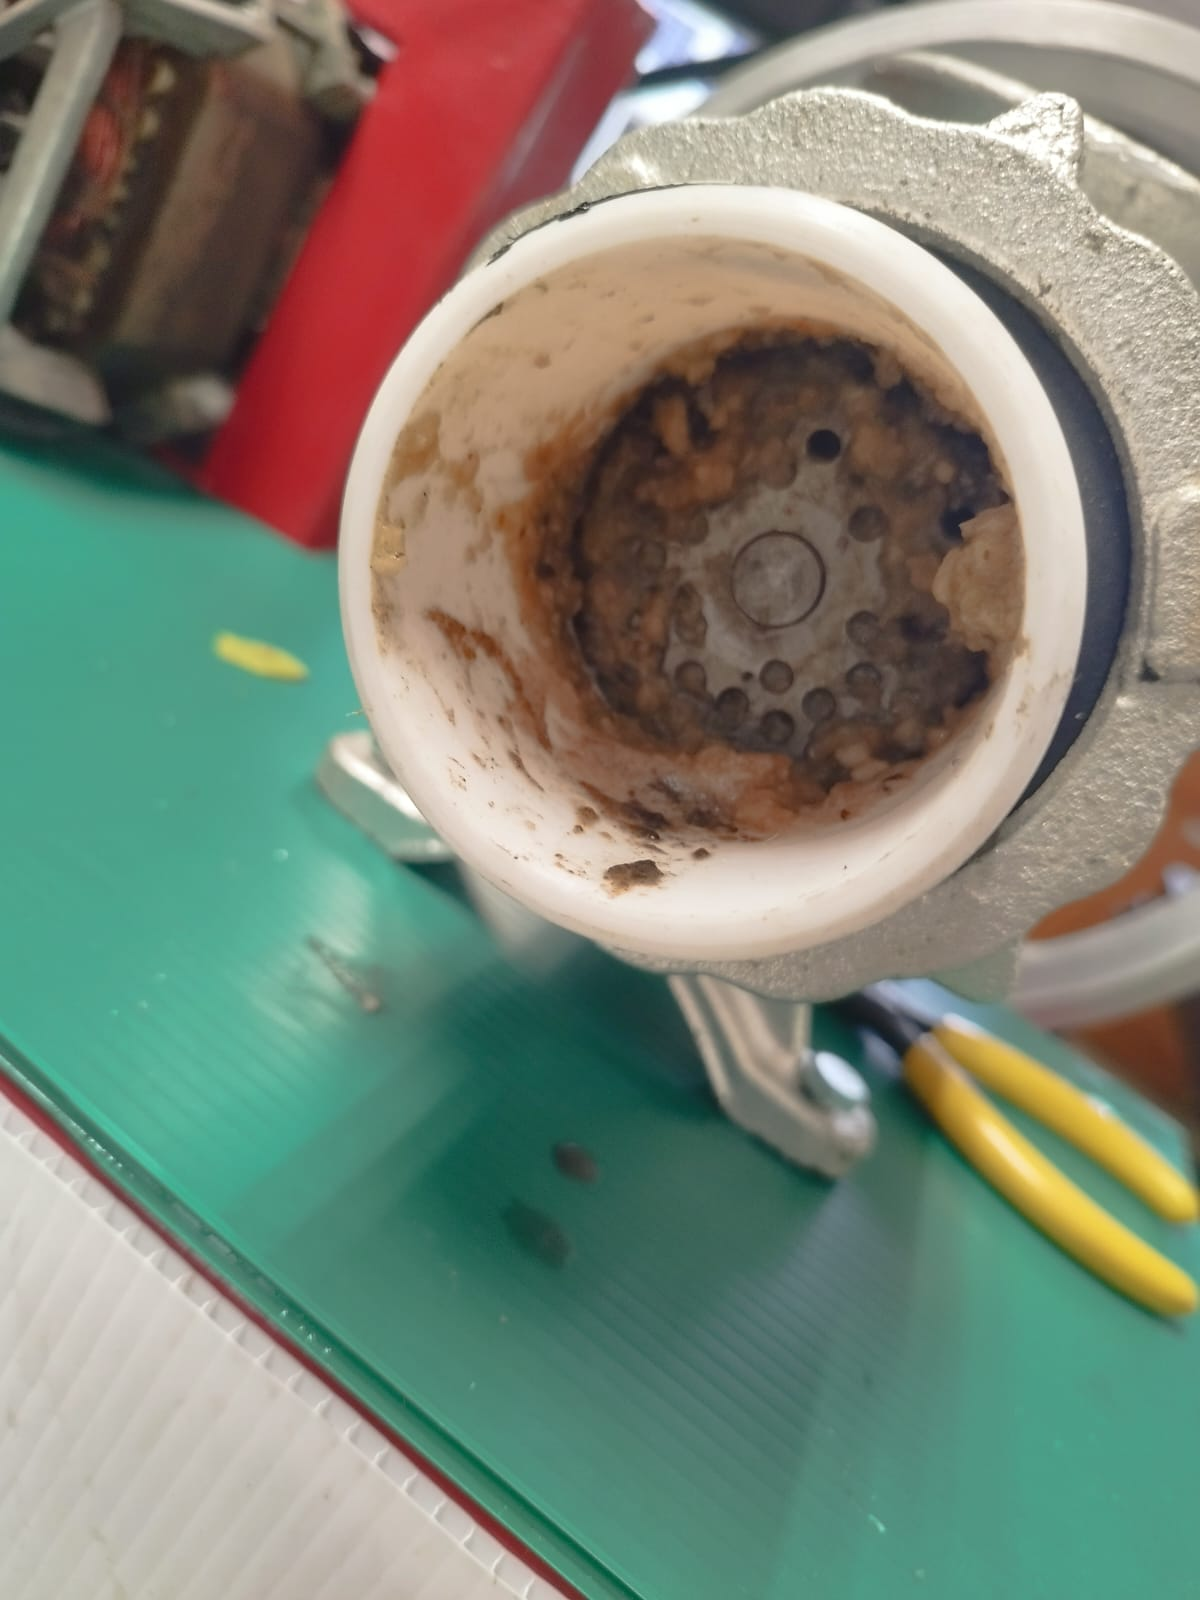
\includegraphics[scale=0.15]{images/Capitulo_Imple/S7/atorado.jpeg}
            \caption{Triturador atascado}
            \label{fg:Atasco tritu}
 \end{figure}
 
Para el caso de las hojas de lechuga, los tallos de cebollas, las cáscaras de zanahoria y melón, el sistema de trituración no era eficiente. Debido a que son elementos delgados y largos que se quedan atrapados alrededor del tornillo sin fin o en las paredes del molino.

El resultado de esta prueba fue de ayuda para delimitar el tamaño de los residuos a la entrada de la trituración. Estos deben estar en un rango de 1 a 3 cm de largo por 1 a 3 cm de ancho. Tampoco se le deben introducir tallos enteros ni cáscaras.
 
Para la segunda prueba de trituración, se utilizaron residuos de papa, zanahoria, sandía, melón y jícama. Estos elementos fueron previamente picados para cumplir con el requerimiento de entrada.

Con las muestras picadas, se procedió a introducir los desechos al triturador. Esto se hizo de forma lenta para evitar que se atascaran.

Este proceso llevó a mejores resultados, moler todos los residuos provoco un par de pequeños atascos, sin embargo a diferencia del primer experimento no generó más problemas.

De esta manera, se obtuvo una materia molida a través de un cedazo con aberturas de 3 mm (Figura \ref{fg:Mat tritu}), por lo que la materia se comenzó a almacenar dentro del contenedor.

 \begin{figure}[h]
            \centering
            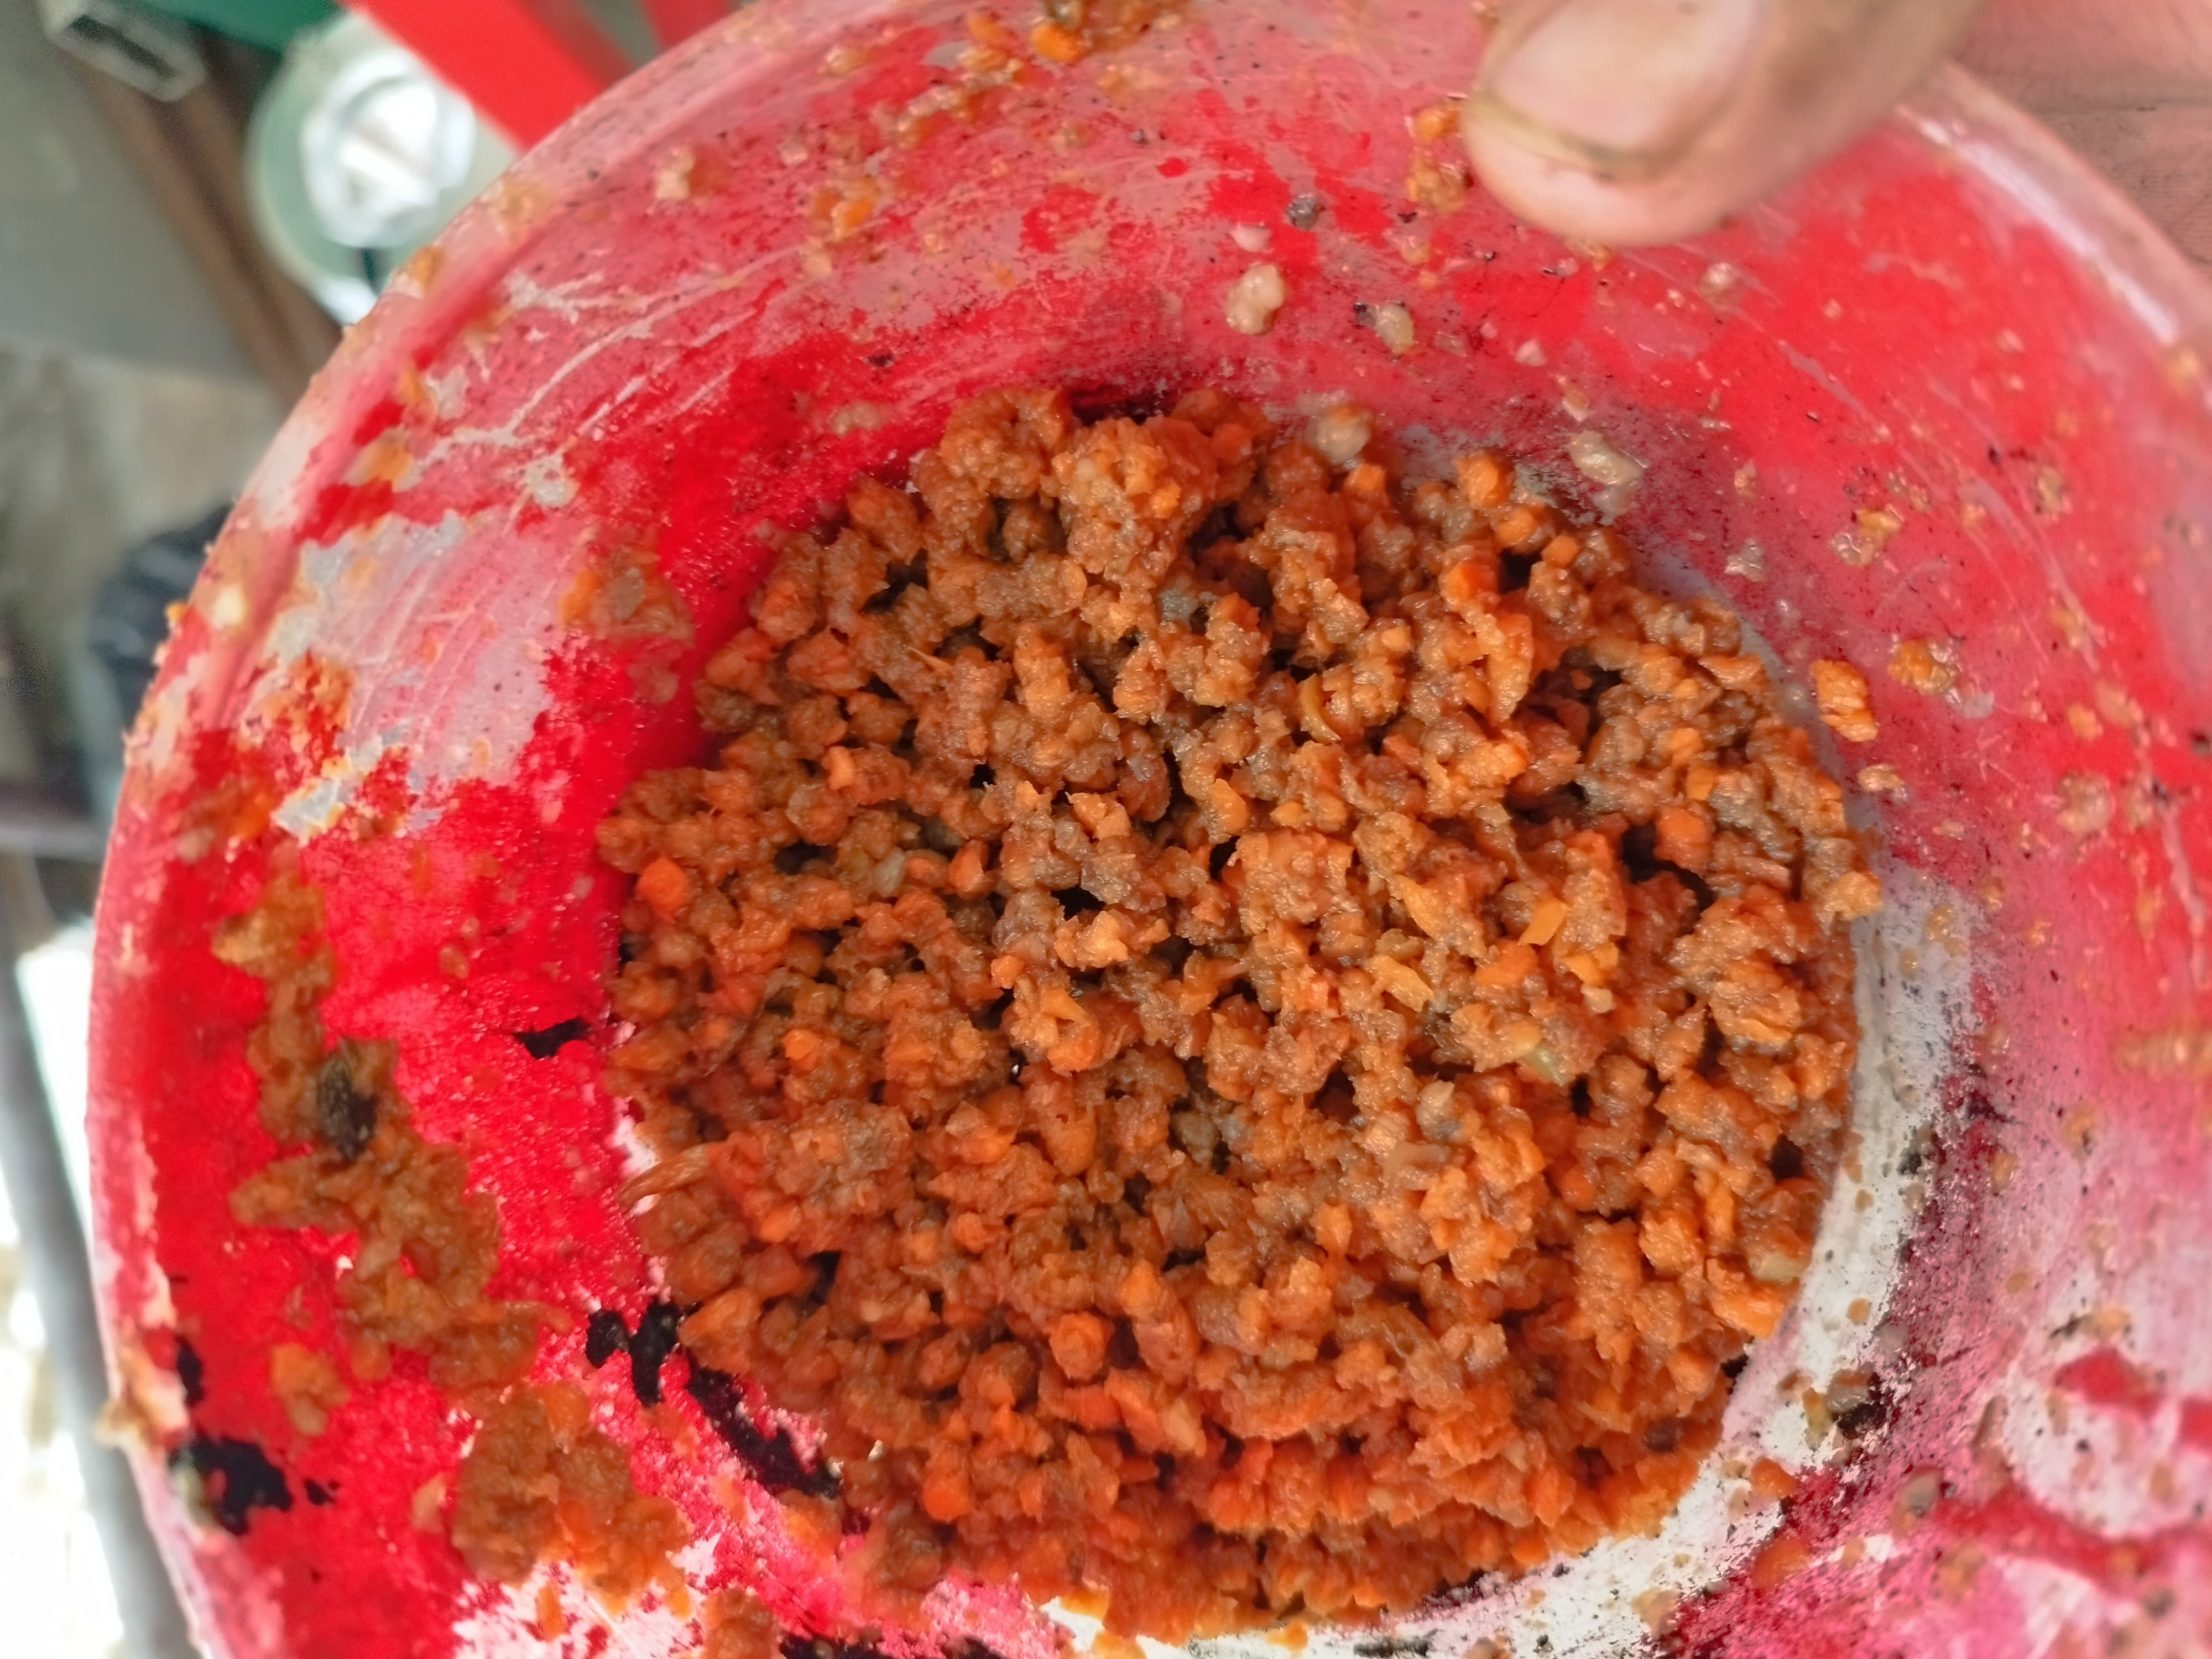
\includegraphics[scale=0.073]{images/Capitulo_Imple/S7/triturado.jpeg}
            \caption{Materia recién salida del triturador}
            \label{fg:Mat tritu}
 \end{figure}
 
 \clearpage
 
Por otro lado, estas pruebas permitieron notar que el adaptador que conecta al triturador con la estructura de PVC también contribuía con el atascamiento de la materia triturada, ya que el diámetro interior no era del tamaño adecuado. Al revisar el triturado de los vegetales, el equipo se percató de que la mayor parte de la materia sale por los orificios más cercanos al perímetro del cedazo.

Por tal motivo, fue necesario diseñar otra pieza que permitiera el paso de la materia mediante un diámetro mayor, pero que, al mismo tiempo, pudiera conectarse con la estructura de PVC que ya se tenía construida.

Para solucionar este problema, se pensó en el diseño del un cono excéntrico como el que se muestra a continuación:
 \begin{figure}[h]
            \centering
            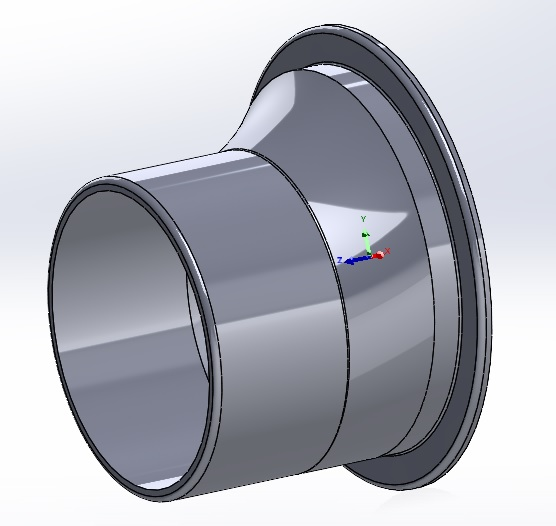
\includegraphics[scale=0.7]{images/Pruebas/Pruebas_S4/cono_excentrico.jpg}
            \caption{Adaptador con cono excéntrico}
            \label{fg:conexcentrico}
 \end{figure}

\clearpage